\chapter{Sequences in Calculus}
\index{sequences}
We introduced sequences in a previous chapter. Now, we will examine them 
in more detail in the context of calculus. You already know about arithmetic and 
geometric sequences, but not all sequences can be classified as arithmetic or 
geometric. Take the famous Fibonacci sequence, \{1, 1, 2, 3, 5, 8, ...\}, 
which can be explicitly defined as $a_n = a_{n-1} + a_{n-2}$, with $a_1 = a_2 
= 1$. There is no common difference or common ratio, so the Fibonacci sequence 
is not arithmetic or geometric. Another example is $a_n = \sin{\frac{n\pi}{6}}$, 
which will cycle through a set of values. 

Sequences have many real-world applications, including compound interest and 
modeling population growth. In later chapters, you will learn that the sum of 
all the values in a sequence is a series and how to use series to describe 
functions. In order to be able to do all that, we first need to talk in depth 
about sequences. 

Some sequences are defined explicitly, like $a_n = \sin{\frac{n\pi}{6}}$, while 
others are defined recursively, like $a_n = a_{n-1} + a_{n-2}$. 

\textbf{Example}: Write the first 5 terms for the explicitly defined sequence $a_n = 
\frac{n}{n+1}$.

\textbf{Solution}: We can construct a table to keep track of our work:
\begin{center}
\begin{tabular}{|c|c|c|}\hline
$n$ & work & $a_n$\\
\hline
1 & $\frac{1}{1+1}$ & $\frac{1}{2}$\\
\hline
2 & $\frac{2}{2+1}$ & $\frac{2}{3}$\\
\hline
3 & $\frac{3}{3+1}$ & $\frac{3}{4}$\\
\hline
4 & $\frac{4}{4+1}$ & $\frac{4}{5}$\\
\hline
5 & $\frac{5}{5+1}$ & $\frac{5}{6}$\\
\hline
\end{tabular}
\end{center}

So, the first five terms are \{$\frac{1}{2}$, $\frac{2}{3}$, $\frac{3}{4}$, 
$\frac{4}{5}$, and $\frac{5}{6}$\}. 

\begin{Exercise}[label = seqcalc1]
Write the first five terms for each sequence. 
\begin{enumerate}
\item $a_n = \frac{2^n}{2n+1}$
\item $a_n = \cos{\frac{n\pi}{2}}$
\item $a_1 = 1$, $a_{n+1} = 5a_n-3$
\item $a_1 = 6$, $a_{n+1} = \frac{a_n}{n+1}$
\end{enumerate}
\end{Exercise}

\begin{Answer}[ref=seqcalc1]
\begin{enumerate}
\item $\frac{2}{3}$, $\frac{4}{5}$, $\frac{8}{7}$, $\frac{16}{9}$, $\frac{32}{11}$
\item 0, -1, 0, 1, 0
\item 1, 2, 7, 32, 157
\item 6, 3, 1, $\frac{1}{4}$, $\frac{1}{20}$
\end{enumerate}
\end{Answer}


\section{Convergence and Divergence}
\index{sequences!divergence}
\index{sequences!convergence}
You can visualize a sequence on an $xy$-plane or a number line. Figures 
\ref{fig:linefrac} and \ref{fig:planefrac} show visualizations of the sequence 
$a_n = \frac{n}{n+1}$. To visualize this on the $xy$-plane, we take points such 
that $x = n$ and $y = a_n$, where $n$ is a positive integer. What do you notice 
about this sequence? As $n$ increases, $a_n$ gets closer and closer to $1$. 

\begin{figure}[htbp]
\centering
    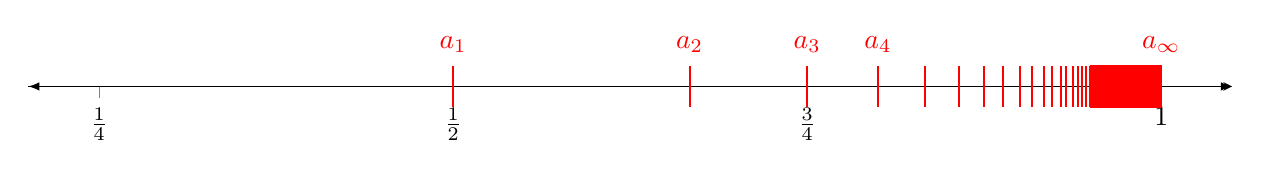
\begin{tikzpicture}
        \begin{axis}[axis y line = none, width = 2*\axisdefaultwidth, 
        height = 0.25*\axisdefaultwidth, axis lines = center, 
        xtick align = outside, xmin = 0.2, xmax = 1.05, 
        xtick = {0.25, 0.5, 0.75, 1}, xticklabels = {$\frac{1}{4}$, 
        $\frac{1}{2}$, $\frac{3}{4}$, $1$}, ymin = -0.5, ymax = 0.5, 
        clip = false]
        \draw[latex-latex](0.2, 0) --(1.05,0);
        \draw[red, thick] (0.5, -0.5) -- (0.5, 0.5);
        \draw[red, thick] (0.667, -0.5) -- (0.667, 0.5);
        \draw[red, thick] (0.75, -0.5) -- (0.75, 0.5);
        \draw[red, thick] (0.8, -0.5) -- (0.8, 0.5);
        \draw[red, thick] (0.833, -0.5) -- (0.833, 0.5);
        \draw[red, thick] (0.857, -0.5) -- (0.857, 0.5);
        \draw[red, thick] (0.875, -0.5) -- (0.875, 0.5);
        \draw[red, thick] (0.888, -0.5) -- (0.888, 0.5);
        \draw[red, thick] (0.9, -0.5) -- (0.9, 0.5);
        \draw[red, thick] (0.909, -0.5) -- (0.909, 0.5);
        \draw[red, thick] (0.917, -0.5) -- (0.917, 0.5);
        \draw[red, thick] (0.923, -0.5) -- (0.923, 0.5);
        \draw[red, thick] (0.929, -0.5) -- (0.929, 0.5);
        \draw[red, thick] (0.933, -0.5) -- (0.933, 0.5);
        \draw[red, thick] (0.9375, -0.5) -- (0.9375, 0.5);
        \draw[red, thick] (0.941, -0.5) -- (0.941, 0.5);
        \draw[red, thick] (0.944, -0.5) -- (0.944, 0.5);
        \draw[red, thick] (0.947, -0.5) -- (0.947, 0.5);
        \draw[red, thick] (0.95, -0.5) -- (0.95, 0.5);
        \filldraw[red](0.95, -0.5) rectangle (1, 0.5);
        \node[red] at (0.5, 1) {$a_1$};
        \node[red] at (0.667, 1) {$a_2$};
        \node[red] at (0.75, 1) {$a_3$};
        \node[red] at (0.8, 1) {$a_4$};
        \node[red] at (1, 1) {$a_{\infty}$};
        \end{axis}
\end{tikzpicture}
    \caption{$a_n =\frac{n}{n+1}$ on a number line}
    \label{fig:linefrac}
\end{figure}

\begin{figure}[htbp]
\centering
    \begin{tikzpicture}
        \begin{axis}[axis lines = center, xmin = -0.5, xmax = 15, 
        ymin = -0.5, ymax = 1.5, xlabel=$n$, ylabel = $a_n$]
        \addplot[blue, dashed] coordinates {(0, 1) (15, 1)};
        \addplot[mark=*, red] (1, 0.5);
        \addplot[mark=*, red] (2, 0.667);
        \addplot[mark=*, red] (3, 0.75);
        \addplot[mark=*, red] (4, 0.8);
        \addplot[mark=*, red] (5, 0.833);
        \addplot[mark=*, red] (6, 0.857);
        \addplot[mark=*, red] (7, 0.875);
        \addplot[mark=*, red] (8, 0.888);
        \addplot[mark=*, red] (9, 0.9);
        \addplot[mark=*, red] (10, 0.909);
        \addplot[mark=*, red] (11, 0.917);
        \addplot[mark=*, red] (12, 0.923);
        \addplot[mark=*, red] (13, 0.929);
        \addplot[mark=*, red] (14, 0.933);
        \addplot[mark=*, red] (15, 0.9375);
        \end{axis}
\end{tikzpicture}
    \caption{$a_n =\frac{n}{n+1}$ on an $xy$-plane}
    \label{fig:planefrac}
\end{figure}

Because $a_n$ approaches a specific number as $n \to \infty$, we call the 
series $a_n = \frac{n}{n+1}$ \textit{convergent}. We prove a sequence is 
convergent by taking the limit as $n$ approaches $\infty$. If the limit exists 
and approaches a specific number, the sequence is convergent. If the limit 
does not exist or approaches $\pm\infty$, the sequence is divergent. 

We can see graphically that $\lim_{n \to \infty} \frac{n}{n+1} = 1$, so that 
sequence is convergent. What about $b_n = \frac{n}{\sqrt{10 + n}}$? Is $b_n$ 
convergent or divergent? 
$$\lim_{n \to \infty} \frac{n}{\sqrt{10 + n}} = 
\lim_{n \to \infty} \frac{n/n}{\sqrt{\frac{10}{n^2}+ \frac{n}{n^2}}}$$
$$=\lim_{n \to \infty} \frac{1}{\sqrt{\frac{10}{n^2}+\frac{1}{n}}} = \infty$$

Therefore, the sequence $b_n = \frac{n}{\sqrt{10 + n}}$ is divergent. 

Here is another example of a divergent sequence: $c_n = \sin{\frac{n\pi}{2}}$. 
The graph is shown in figure \ref{fig:sineseq}. As you can see, the value of 
$c_n$ oscillates between 1, 0, and -1 without approaching a specific number. 
This means that $c_n$ does not approach a particular number as $n \to \infty$ 
and the sequence is divergent. 

\begin{figure}[htbp]
\centering
    \begin{tikzpicture}
        \begin{axis}[axis lines = center, xmin = -0.5, xmax = 8, 
        ymin = -1.5, ymax = 1.5, xlabel=$n$, ylabel = $c_n$]
        \addplot[mark=*, red] (1, 1);
        \addplot[mark=*, red] (2, 0);
        \addplot[mark=*, red] (3, -1);
        \addplot[mark=*, red] (4, 0);
        \addplot[mark=*, red] (5, 1);
        \addplot[mark=*, red] (6, 0);
        \addplot[mark=*, red] (7, -1);
        \addplot[mark=*, red] (8, 0);
        \end{axis}
\end{tikzpicture}
    \caption{$c_n =\sin{\frac{n\pi}{2}}$ on an $xy$-plane}
    \label{fig:sineseq}
\end{figure}

\begin{Exercise}[label=seqcalc3]
Classify each sequence as convergent or divergent. If the sequence is 
convergent, find the limit as $n \to \infty$.
\begin{enumerate}
\item $a_n = \frac{3 + 5n^2}{n + n^2}$
\item $a_n = \frac{n^4}{n^3 - 2n}$
\item $a_n = 2 + (0.86)^n$
\item $a_n = \cos{\frac{n\pi}{n+1}}$
\item $a_n = \sin{n}$
\end{enumerate}
\end{Exercise}

\begin{Answer}[ref=seqcalc3]
\begin{enumerate}
\item convergent, 5
\item divergent
\item convergent, 2
\item convergent, -1
\item divergent
\end{enumerate}
\end{Answer}

\section{Evaluating limits of sequences}\index{sequences!limits of}
Recall that a sequence can be considered a function where the domain is 
restricted to positive integers. If there is some $f(x)$ such that $a_n = f(n)$ 
when $n$ is an integer, then $\lim_{n \to \infty} a_n = \lim_{x \to \infty} 
f(x)$ (see figure \ref{fig:limit}). This means that all the rules that apply to 
the limits of functions also apply to the limits of sequences, including the 
Squeeze Theorem and l'Hospital's rule. 

\textbf{Example}: What is $\lim_{n \to \infty} \frac{\ln{n}}{n}$? 

\textbf{Solution}: First, we will try to compute the limit directly:
$$\lim_{n \to \infty} \frac{\ln{n}}{n} = $$
$$\frac{\lim_{n \to \infty} \ln{n}}{\lim_{n \to \infty}n} = 
\frac{\infty}{\infty}$$

This is undefined, but fits the criteria for L'Hospital's rule:
$$\lim_{n \to \infty} \frac{\ln{n}}{n} = \lim_{n \to \infty} 
\frac{\frac{d}{dn}\ln{n}}{\frac{d}{dn}n}$$
$$= \lim_{n \to \infty} \frac{\frac{1}{n}}{1} = 0$$

\begin{figure}[htbp]
\centering
    \begin{tikzpicture}
        \begin{axis}[axis lines = center, xmin = -0.5, xmax = 8.5, 
        ymin = 0, ymax = 2, xlabel=$n$, ylabel = $a_n$]
        \addplot[mark=*, red] (1, 2);
        \addplot[mark=*, red] (2, 1.5);
        \addplot[mark=*, red] (3, 1.333);
        \addplot[mark=*, red] (4, 1.25);
        \addplot[mark=*, red] (5, 1.2);
        \addplot[mark=*, red] (6, 1.167);
        \addplot[mark=*, red] (7, 1.143);
        \addplot[mark=*, red] (8, 1.125);
        \draw[blue, dashed, thin] (0, 1) -- (8, 1);
        \addplot[red, domain = 0.01:8] {1+1/x};
        \end{axis}
\end{tikzpicture}
    \caption{The limit of the function is the same as the limit of the sequence}
    \label{fig:limit}
\end{figure}

\textbf{Example}: Is the sequence $a_n = \frac{n!}{n^n}$ convergent or divergent? 

\textbf{Solution}: First trying to take the limit directly, we see that:
$$\lim_{n \to \infty} \frac{n!}{n^n} = \frac{\infty}{\infty}$$

which is undefined. Because the factorial cannot be described as a continuous 
function, we can't use L'Hospital's rule. We can examine this sequence 
graphically (see figure \ref{fig:factorial}) and mathematically. We examine it 
mathematically by writing out a few terms to get an idea of what happens to 
$a_n$ as $n$ gets large:
$$a_1 = \frac{1!}{1^1} = 1$$
$$a_2 = \frac{2!}{2^2} = \frac{1 \cdot 2}{2 \cdot 2}$$
$$a_3 = \frac{3!}{3^3} = \frac{1 \cdot 2 \cdot 3}{3 \cdot 3 \cdot 3}$$
$$\cdots$$
$$a_n = \frac{n!}{n^n} = \frac{1 \cdot 2 \cdot 3 \cdots \cdot n}{n 
\cdot n \cdot n \cdots n}$$

From examining the graph in figure \ref{fig:factorial}, we can guess that 
$\lim_{n \to \infty} a_n = 0$. Let's prove that mathematically. We can rewrite 
our expression for $a_n$ as $n$ gets larger:
$$a_n = \frac{n!}{n^n} = \frac{1 \cdot 2 \cdot 3 \cdots \cdot n}{n 
\cdot n \cdot n \cdots n} = \frac{1}{n}(\frac{2 \cdot 3 \cdots n}{n 
\cdot n \cdots n})$$

The expression inside the parentheses is less than 1; therefore, $0 < a_n < 
\frac{1}{n}$. Since $lim_{n \to \infty} 0 = 0$ and $\lim_{n \to \infty} 
\frac{1}{n} = 0$, by Squeeze Theorem, we know that $\lim_{n \to \infty} 
\frac{n!}{n^n} = 0$. Therefore, the sequence $a_n = \frac{n!}{n^n}$ is 
convergent. 

\begin{figure}[htbp]
\centering
    \begin{tikzpicture}
        \begin{axis}[axis lines = center, xmin = -0.5, xmax = 8.5, 
        ymin = 0, ymax = 1, xlabel=$n$, ylabel = $a_n$]
        \addplot[mark=*, red] (1, 1);
        \addplot[mark=*, red] (2, 0.5);
        \addplot[mark=*, red] (3, 0.222);
        \addplot[mark=*, red] (4, 0.09375);
        \addplot[mark=*, red] (5, 0.0384);
        \addplot[mark=*, red] (6, 0.01543);
        \addplot[mark=*, red] (7, 0.00612);
        \addplot[mark=*, red] (8, 0.0024);
        \end{axis}
\end{tikzpicture}
    \caption{$a_n = \frac{n!}{n^n}$}
    \label{fig:factorial}
\end{figure}

[[FIX ME intro]]
If $\lim_{n \to \infty} a_n = L$ and the function $f$ is continuous at $L$, 
then $\lim_{n \to \infty} f(a_n) = f(L)$. For example, what is $\lim_{n \to 
\infty} \sin{\frac{\pi}{n}}$? Well, we know that $\lim_{n \to \infty} 
\frac{\pi}{n} = 0$ and that the sine function is continuous at 0. Therefore, 
$\lim_{n \to \infty} \sin{\frac{\pi}{n}} = \sin{\lim_{n \to \infty} 
\frac{\pi}{n}} = \sin{0} = 0$. 

\section{Monotonic and Bounded sequences}
\index{sequences!monotonic}
\index{sequences!bounded}
Just like functions, sequences can be increasing or decreasing. A sequence is 
increasing if $a_n < a_{n+1}$ for $n \geq 1$. Similarly, a sequence is 
decreasing if $a_n > a_{n+1}$ for $n \geq 1$. If a sequence is strictly 
increasing or decreasing, it is called \textit{monotonic}. 

The sequence $a_n = \frac{1}{n + 6}$ is decreasing. We prove this formally by 
comparing $a_n$ to $a_{n+1}$:
$$\frac{1}{n + 6} > \frac{1}{(n + 1) + 6} = \frac{1}{n + 7}$$

\textbf{Example}: Is the sequence $a_n = \frac{n}{n^2 + 1}$ increasing or 
decreasing? 

\textbf{Solution}: First, we find an expression for $a_{n+1}$:
$$a_{n + 1} = \frac{n + 1}{(n + 1)^2 + 1} = \frac{n + 1}{n^2 + 2n + 2}$$

Since the degree of $n$ is greater in the denominator, we have a guess that 
the sequence is decreasing. To prove this, we check if $a_n > a_{n+1}$ is true:
$$\frac{n}{n^2 + 1} > \frac{n + 1}{n^2 + 2n + 2}$$

We can cross-multiply, because $n > 0$ and the denominators are positive:
$$(n)(n^2 + 2n + 2) > (n+1)(n^2 + 1)$$
$$n^3 + 2n^2 + 2n > n^3 + n^2 + n + 1$$

Subtracting $(n^3 + n^2 + n)$ from both sides we see that:
$$n^2 + n > 1$$

Which is true for all $n \geq1$. Therefore, $a_n > a_{n+1}$ for all $n \geq 1$ 
and the sequence is decreasing. 

A sequence is \textit{bounded above} if there is some number $M$ such that 
$a_n \leq M$ for all $n \geq 1$. A sequence is \textit{bounded below} if 
there is some other number $m$ such that $a_n \geq m$ for all $n \geq 1$. If a 
sequence is bounded above and below, then it is a \textit{bounded sequence}. 

Not all bounded sequences are convergent. Take our earlier example of $a_n = 
\sin{\frac{n\pi}{6}}$. This sequence is bounded, since we can say that $- 1 
\leq a_n \leq 1$ for all $n$. However, $a_n = \sin{\frac{n\pi}{6}}$ is 
divergent because $\lim_{n \to \infty} \sin{\frac{n\pi}{6}}$ does not exist 
(see figure \ref{fig:divsine}). Additionally, not all monotonic sequences are 
convergent. Consider $b_n = 2^n$ (shown in figure \ref{fig:divexp}). This is 
monotonically increasing (that is, $b_n > b_{n-1}$ for all n), but $\lim_{n \to 
\infty} 2^n = \infty$ and the sequence is divergent. 

\begin{figure}
    \centering
    \begin{tikzpicture}
        \begin{axis}[xmin = -0.5, xmax = 24, ymin = -1.4, ymax = 1.4, 
        ytick = {-1, 1}, axis lines = center, xtick = {4, 8, 12, 16, 20, 24}, 
        xlabel = $n$, clip = false]
        \foreach \n in {1, ..., 24} {
        \addplot[red, mark=*]({\n}, {sin(deg(\n * pi/6))});
        }
        \addplot[blue, dashed, domain = 0:24]{1};
        \addplot[blue, dashed, domain = 0:24]{-1};
        \node[blue] at (3, 1.3) {$M = 1$};
        \node[blue] at (21, -1.3) {$m = -1$};
        \end{axis}
    \end{tikzpicture}
    \caption{The sequence $a_n = \sin{\frac{n\pi}{6}}$ is bounded and divergent}
    \label{fig:divsine}
\end{figure}

\begin{figure}
    \centering
    \begin{tikzpicture}
        \begin{axis}[xmin = -0.5, xmax = 5, ymin = 0, ymax = 33, 
        axis lines = center, xlabel = $n$, clip = false]
        \foreach \n in {1, ..., 5} {
        \addplot[red, mark=*]({\n}, {2^(\n)});
        }
        \addplot[blue, dashed, domain = 0:5]{2};
        \node[blue] at (5, 5) {$m = 2$};
        \end{axis}
    \end{tikzpicture}
    \caption{The sequence $b_n = 2^n$ is bounded below, monotonically 
    increasing, and divergent}
    \label{fig:divexp}
\end{figure}

A sequence must be convergent if it is \textbf{both} monotonic and bounded. 
Why is this? Recall that to be bounded, a sequence must be bounded above and 
below, which means there is some $m$ and some $M$ such that $m \leq a_n \leq M$ 
for all $n$. If the sequence is increasing, the terms must get close to but not 
exceed $M$. Likewise, if the sequence is decreasing, the terms must get close 
to, but not be less than $m$.

\textbf{Example}: Is the sequence given by $a_1 = 4$ and $a_{n+1} = \frac{1}{2} 
(a_n + 7)$ bounded above, below, both, or neither?

\textbf{Solution}: We start by calculating the first several terms:
\begin{center}
	\begin{tabular}{|c|c|c|}\hline
	Term & Work & Value\\
	\hline
	$a_1$ & $a_1 = 4$ & 4\\
	\hline
	$a_2$ & $=\frac{1}{2}(4 + 7)$ & 5.5\\
	\hline
	$a_3$ & $=\frac{1}{2}(5.5+7)$ & 6.25\\
	\hline
	$a_4$ & $=\frac{1}{2}(6.25+7)$ & 6.625\\
	\hline
	$a_5$ & $=\frac{1}{2}(6.625+7)$ & 6.8125\\
	\hline
	$a_6$ & $=\frac{1}{2}(6.8125+7)$ & 6.90625\\
	\hline
	$a_7$ & $=\frac{1}{2}(6.90625+7)$ & 6.953125\\
	\hline
	$a_8$ & $=\frac{1}{2}(6.953125+7)$ & 6.9765625\\
	\hline	
	\end{tabular}
\end{center}

The sequence is increasing, so it is bounded below by the initial term, $a_1 = 
4$, and we can state that $a_n \geq 4$. Examining the computed terms, we see 
that $a_n \to 7$ as $n$ grows larger. We can guess that this sequence is 
bounded above, with $a_n \leq 7$. We can prove this by induction. Suppose that 
there is some $k$ such that $a_k < 7$ (which is true for $a_1$, etc.). Then,
$$a_k < 7$$
$$a_k + 7 < 14$$
$$\frac{1}{2}(a_k + 7) < \frac{1}{2}(14)$$
$$a_{k + 1} < 7$$\\
Therefore, $a_n < 7$ for all $n$ and the sequence is bounded above. Because 
the sequence is monotonic and bounded, we know the sequence is convergent and, 
therefore, that the limit of $a_n$ as $n \to \infty$ exists. 

\section{Applications of Sequences}
\index{sequences!applications of}
\subsection{Compound Interest}
You previously learned about compound interest and modeled the accumulation of 
compound interest by $P_n = P_0(1 + r)^n$, where $P_0$ is the principal 
investment, $r$ is the yearly interest rate, and $n$ is the number of elapsed 
years. This sequence describes the value of an investment accumulating 
interest, but most people add to their savings on a regular schedule. We can 
write a sequence to model the value of a savings account that the owner makes 
regular deposits into. 

\textbf{Example}: Suppose you open a savings account with an initial deposit 
of \$3,000 and you plan to deposit an additional \$1,200 at the end of every 
year. If your savings account has an annual interest rate of 3.25\%, how long 
will it take you to save \$10,000?

\textbf{Solution}: We can write a recursive definition for the sequence. At 
the end of each year, the account will gain the interest on the entirety of 
the previous year's balance plus \$1200:
$$P_n = P_{n-1}(1+0.0325) + \$1200$$\\
With an initial investment $P_0 = \$3000$. We can write out the first few terms 
to find how many years it will take to save \$10,000:
\begin{center}
\begin{tabular}{|c|c|}\hline
Year & Savings\\
\hline
0 & \$3,000\\
\hline
1 & \$4,297.50\\
\hline
2 & \$5,637.17\\
\hline
3 & \$7,020.38\\
\hline
4 & \$8,448.54\\
\hline
5 & \$9.923.12\\
\hline
6 & \$11,445.62\\
\hline
\end{tabular}
\end{center}

The accumulation of interest with deposits is better described by a sequence than a function. That iss because the deposits are happening at discrete times, not continuously. 

\begin{Exercise}[label=seqcalc5]
You invest \$1500 at 5\%, compounded annually. Write an explicit formula that 
describes the value of your investment every year. What will your investment 
be worth after 10 years? Is the sequence convergent or divergent? Explain. 
\end{Exercise}

\begin{Answer}[ref=seqcalc5]
Out principal is $P = 1500$ and the interest rate is $r = 0.06$. After $n$ 
years, your investment will be worth $a_n = 1500(1.06)^{n}$. For $n = 10$, 
your investment will be valued at $a_{10} = \$1500(1.06)^{10} = \$2686.27$ 
(that's over \$1000 in interest!). To determine if the sequence is convergent 
or divergent, we examine the limit as $n \to \infty$:
$$\lim_{n \to \infty} 1500(1.06)^n = 1500\cdot \lim_{n \to \infty}
(1.06)^n = 1500 \cdot \infty = \infty$$\\
The sequence is divergent. 
\end{Answer}

\subsection{Population Growth}
Sequences can be used to model a reproducing population that is being 
occasionally culled from or added to. Similar to compound interest, a 
population of living things (plants, animals, fungi, etc.) reproducing at a 
rate \textit{r} can be modeled with an exponential function:
$$P_n = P_0(1+r)^n$$\
where $P_0$ is the initial population, $r$ is the yearly reproductive rate, 
and $n$ is the number of years elapsed. 

\textbf{Example}: Suppose the population of deer in a national park is 
estimated to be 6,500. If the deer reproduce at a rate of 8\% per year and 
wolves hunt and kill 500 deer per year, how many deer will be in the park in 5 
years? 

\textbf{Solution}: We can write a recursive sequence:
$$P_n = P_{n-1}(1 + 0.08) - 500$$
$$P_0 = 6500$$
And calculate $P_5$ (we round to the nearest whole number because half of a 
deer is not a living deer):
\begin{center}
\begin{tabular}{|c|c|c|}\hline
Year & & Population\\
\hline
1 & $6500(1.08) - 500$ & 6520\\
\hline
2 & $6520(1.08) - 500$ & 6542\\
\hline
3 & $6542(1.08) - 500$ & 6565\\
\hline
4 & $6565(1.08) - 500$ & 6590\\
\hline
5 & $6590(1.08) - 500$ & 6617\\
\hline
\end{tabular}
\end{center}
There will be 6617 deer in the park after 5 years. 

\begin{Exercise}[label=seqcalc6]
A farmer keeps his pond stocked with fish. If the fish are eaten by predators 
at a rate of 5\% per month and the farmer can afford to restock the pond with 
10 fish every 6 months. If the farmer starts with 100 fish, how many total fish 
will he have lost to predation after 4 years?
\end{Exercise}

\begin{Answer}[ref=seqcalc6]
The number of fish in the pond is:
$$P_n = P_{n-1}(0.95)^6 + 50$$
$$P_0 = 100$$\\
where $n$ is the number of 6-month periods that have passed. The four-year 
period is given by $1 \leq n \leq 8$. The amount lost to predation every 6 
months is given by $P_{n-1}(1-0.95^6)$.
\begin{center}
\begin{tabular}{|c|c|c|}\hline
$n$ & Fish Population & Lost to Predators\\
0 & 100 & \\
\hline
1 & 84 & 26\\
\hline
2 & 71 & 22\\
\hline
3 & 62 & 19\\
\hline
4 & 56 & 17\\
\hline
5 & 51 & 15\\
\hline
6 & 48 & 14\\
\hline
7 & 45 & 13\\
\hline
8 & 43 & 12\\
\hline

\end{tabular}
\end{center}
Adding up all the fish lost to predators, we find that over 4 years, the farmer loses 138 fish. 
\end{Answer}






%FIXME summary section -- comparing exponents and growth rates
